\chapter{Introduction}
\label{sec:introduction}

\section{Problem statement}
\label{sec:prob_stmt}

\begin{figure}
  \centering
  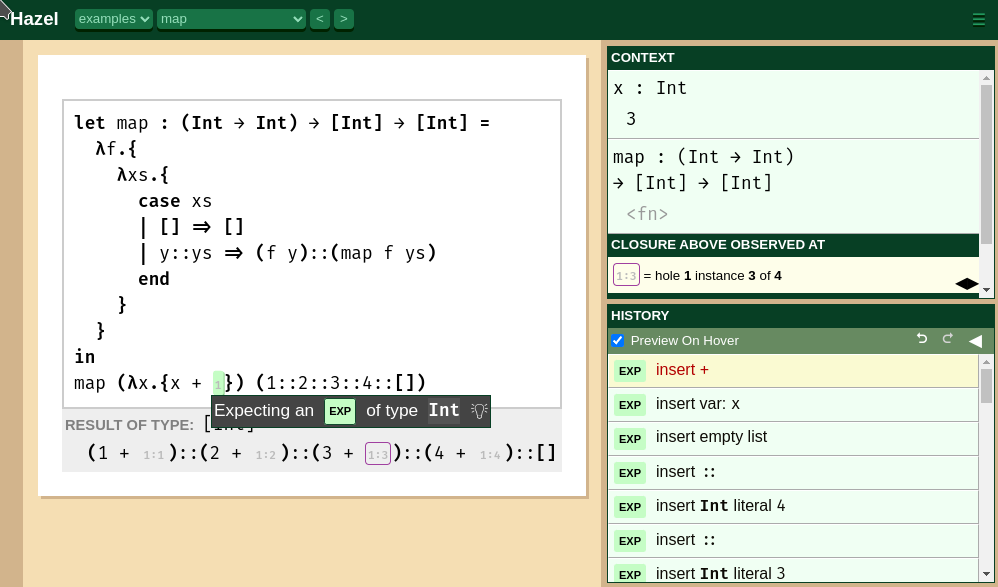
\includegraphics[width=4in]{img/hazel_ui.png}
  \caption[Screenshot of the Hazel live programming environment.]{A screenshot of the Hazel live programming environment. Screenshot taken of the dev branch demo on 02/06/2022 \cite{HazelDemo2022}.}
  \label{fig:screenshot-hazel-ui}
\end{figure}

Unstructured plaintext editing has remained the dominant mode of programming for decades, but makes it more difficult to implement editor services to aid the process. Structural editors, on the other hand, only allow valid edit states. Several structural editors, such as Scratch \cite{maloney2010scratch}, Lamdu \cite{lotem_chuchem}, and mbeddr \cite{voelter2012mbeddr}, have been proposed to improve the programming experience and introduce editor services, such as the elimination of syntax errors or graphical editing.

Hazel \cite{Hazel2022} is an experimental structural language definition and implementation that aims to solve the ``gap problem'': spatial and temporal holes that temporarily prevent code from being able to be compiled or evaluated. The structural editor is defined by a bidirectional edit calculus Hazelnut \cite{conf/popl/Hazelnut17}, which governs the structural editor and the static semantics (typing rules) of the language. The dynamic semantics (evaluation semantics) are described in Hazelnut Live \cite{conf/popl/HazelnutLive19}.

Hazel is a relatively new research effort by the University of Michigan's Future of Programming Lab (FPLab), with little effort placed on performance optimizations. This work attempts to achieve several enhancements to Hazelnut Live that will benefit the performance of evaluation and related tasks. Part of the work will be focused on transitioning the evaluation model from using substitution for variable bindings to using environments, with emphasis on evaluation of holes and postprocessing of the evaluation result to match the result from evaluation with substitution. The latter parts of this work will use the environment model of evaluation to improve the memoization of certain tasks specific to Hazel (such as hole closure numbering), and also implement the fill-and-resume performance enhancement described in \cite{conf/popl/HazelnutLive19}. The novelty of this work lies in the optimization capacity in the unique design of the Hazel language as a live programming editor with expression holes.

\section{The contribution of this work}
\label{sec:contribution}

This thesis presents several algorithms designed for Hazel's evaluation. These algorithms are provided using the big-step inference semantics notation introduced in \Cref{sec:semantics-notation}.

Firstly, we provide the evaluation semantics of the Hazel language using the environment model. We aim to keep the implementation pure, introduce uniquely-numbered environments (for later use in memoization), and describe the evaluation of holes (which are unique to Hazel). We introduce the concepts of generalized closures, and the evaluation boundary.

Secondly, we describe the postprocessing algorithm, which is mostly memoized by environments and has the two major functions. The first is to convert the result to the equivalent result if substitution was used. The second is to number hole closure instances.

Lastly, we develop the fill-and-resume process, as originally proposed (but not implemented) in \cite{conf/popl/HazelnutLive19}. We provide a possible implementation, including an algorithm to detect a valid fill operation and advice on memoizing the resumption operation.

The performance of this work is measured primarily in terms of empirical performance gains (via evaluation-step counting and benchmarking), and discussed with respect to the theoretical performance. Hazelnut \cite{conf/popl/Hazelnut17} and Hazelnut Live \cite{conf/popl/HazelnutLive19} mechanize proofs of their work using the Agda interactive proof checker. We do not provide mechanized proofs of our work; instead, we provide a series of core metatheorems describing invariants describing Hazel evaluation, and argue the correctness of these metatheorems by informal reasoning on the provided inference rules. A mechanized proof using Agda is deferred for future work.

\section{Structural overview}
\label{sec:structural_overview}

\Cref{sec:prog_lang_principles} provides a background on necessary topics in programming language (PL) theory and programming language implementations, in order to frame the understanding for the Hazel live programming environment. \Cref{sec:hazel} provides an overview of Hazel, in order to frame the work completed for this thesis project. \Crefrange{sec:env_model_evaluation}{sec:far_impl} describe the primary work completed for this project, as described in \Cref{sec:contribution}. \Cref{sec:evaluation} comprises an emprical performance assessment of the work. \Cref{sec:discussion} is a discussion of theoretical results. \Cref{sec:future_work} describes unfinished work and future research directions. \Cref{sec:concl} concludes with a summary of findings and future work. The Appendices contain extra inference rules and selected source code snippets.

%%% Local Variables:
%%% mode: latex
%%% TeX-master: "main"
%%% End:
